\section{Simulation Studies} \label{sec:simulation}

In this Section, we present two simulations, one in three dimensions
and the other in seven, in which the target functions were built to
be difficult to integrate, but their shapes can be inferred through
their mathematical expressions. The objective of the simulation
study is to evaluate the efficiency of the importance function
yielded by AAIS, via comparing its shape with that of the real
target, and comparing the calculated marginal likelihood with the
real answer.

\subsection{Three Dimensional Flared
Helix}\label{sec:example1}

We used a cylindrical function with standard Gaussian cross-section
(in ($x$, $y$)) that has been deformed (in $z$) into a helix with
varying diameter. The helix performs three complete turns. The
target function is defined to be
\begin{equation}\label{helix_func}
p(x,y,z)=\delta(-30<z\leq30)\mathcal{N}([x,y]|\mu,\Sigma)
\end{equation}
where $\mu(1)=(z+35)\times\cos(\beta)$ and
$\mu(2)=(z+35)\times\sin(\beta)$, where $\beta=(z+30)\times\pi/10$.
Here $\Sigma=\mbox{diag}([1,1])$. Fig.\ref{fig:flared_helix_target}
shows the shape of this function. And the integration of this
function is shown to be
\begin{equation}
\int\int\int p(x,y,z)dxdydz=\int\int\int p(x,y|z)dxdy
p(z)dz=\int_{-30}^{30} 1 dz=60
\end{equation}
Treating (\ref{helix_func}) to be $L(y|\theta)p(\theta)$, the
marginal likelihood in this simulation case is then 60.

\begin{figure}[!htb]
\centerline{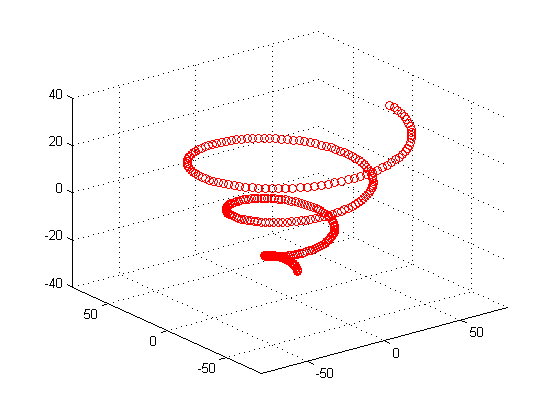
\includegraphics[width=3in,height=2.4in]{Fig/flared_helix_target}}
\caption{The simulated 3-D flared helix target distribution}
\label{fig:flared_helix_target}
\end{figure}
Before running the proposed Adaptive Annealed IS (AAIS) algorithm,
we select the initial proposal to be a T-mixture that is composed of
10 equally weighted components. The degree of freedom for each T
component is fixed to be 5. The centers of these components are
selected uniformly from a region restricted by
$x\in[-100,100],y\in[-100,100]$ and $z\in[-30,30]$. Then the
covariance matrix for every component is identical to
$\mbox{diag}[\sigma_x^2,\sigma_y^2,\sigma_z^2]$, where $\sigma_a$ is
the standard error of the argument $a$ in the components' centers
that has been just specified. The particle size $N=2000$,
$\lambda_t=0.1t$, and $t=1,\ldots,10$.

The adaptive mixture importance sampling (AMIS) approach
\cite{cappe2008ais} is involved for performance comparison. We
initialize it using the same setting as for the AAIS, and let it run
10 iterations to give the final mixture importance function.

Fig. \ref{fig:helix_scatter} shows the resulting posterior samples
(which are equally weighted via resampling) corresponding to AAIS
and AMIS, respectively. It's shown that the samples resulted from
AAIS are distributed in wider posterior area, which indicates that
the importance function given by AAIS captures more structures in
the posterior.

\begin{figure}[!htb]
\begin{tabular}{c}
\centerline{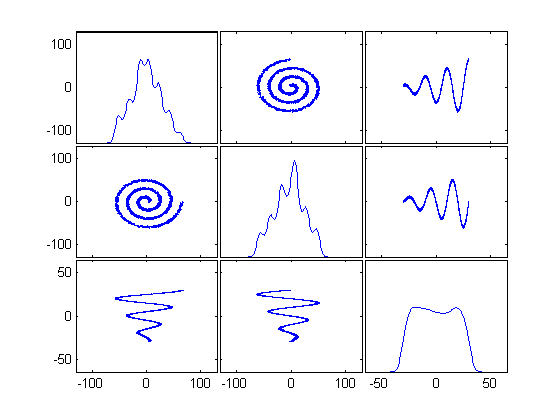
\includegraphics[width=3in,height=2.4in]{Fig/flared_helix_scatter.png}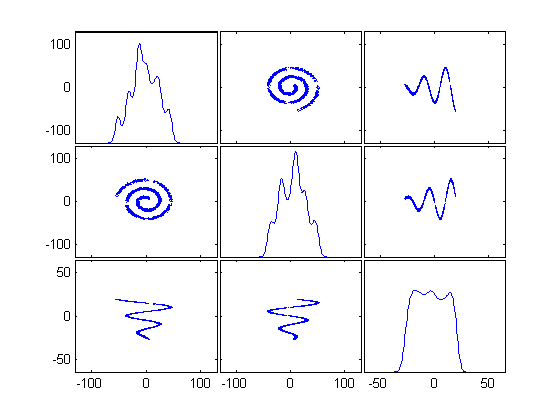
\includegraphics[width=3in,height=2.4in]{Fig/AIS_3d_felix_scatter.png}}
\end{tabular}
\caption{Three dimensional flared helix example. Left:posterior
samples produced by the proposed AAIS algorithm. Right:posterior
samples produced by the AMIS algorithm \citep{cappe2008ais}. In the
diagonal, the curves are kernel density estimates of the posterior
samples.} \label{fig:helix_scatter}
\end{figure}

A quantitative comparison between the importance functions obtained
by AAIS and AMIS is shown in Table \ref{comparison_3D}. Three
quantities are used for comparison, that are the \ESS, the KL
distance and the estimated marginal likelihood. Note that, we can
easily calculate the KL distance via a simple Monte Carlo for this
simulation case. As is shown in Table \ref{comparison_3D}, AAIS
gives correct answer to the marginal likelihood, closer KL distance
with respect to the real target, and bigger \ESS. So it further
demonstrates that the AAIS is much better than the AMIS in dealing
with this simulation case.

\begin{table}
\begin{tabular}{c||c|c|c}
 & \ESS/N & $\KL$ & Marginal Likelihood (real answer:60) \\
\hline AMIS \citep{cappe2008ais} & 0.1525 & 6.7830 & $47.2\pm3.3$\\
\hline AAIS proposed here & 0.4459 & 0.1586 & $59.7\pm2.0$\\
\hline
\end{tabular}
\caption{Three dimensional flared helix example. Quantitative
Performance comparison.}\label{comparison_3D}
\end{table}

\subsection{ Outer Product of Seven Univariate Densities}
To test the concern whether good results from a 3-D example imply
good results in higher dimensions, we used as a target function the
outer product of seven univariate distributions normalized to
integrate to 1. These seven distributions are:
\begin{enumerate}
\item $\frac{3}{5}\mathcal{G}(10+x|2,3)+\frac{2}{5}\mathcal{G}(10-x|2,5)$
\item $\frac{3}{4}sk\mathcal{N}(x|3,1,5)+\frac{1}{4}sk\mathcal{N}(x|-3,3,-6)$
\item $\mathcal{S}(x|0,9,4)$
\item $\frac{1}{2}\mathcal{B}(x+3|3,3)+\frac{1}{2}\mathcal{N}(x|0,1)$
\item $\frac{1}{2}\varepsilon(x|1)+\frac{1}{2}\varepsilon(-x|1)$
\item $sk\mathcal{N}(x|0,8,-3)$
\item $\frac{1}{8}\mathcal{N}(x|-10,0.1)+\frac{1}{4}\mathcal{N}(x|0,0.15)+\frac{5}{8}\mathcal{N}(x|7,0.2)$
\end{enumerate}
Here $\mathcal{G}(\cdot|\alpha,\beta)$ denotes the gamma
distribution, $\mathcal{N}(\cdot|\mu,\sigma)$ denotes the normal
distribution, $sk\mathcal{N}(\cdot|\mu,\sigma,\alpha)$ denotes the
skew-normal distribution, $\mathcal{S}(\cdot|\mu,s,df)$ denotes the
student-T distribution, $\mathcal{B}(\cdot|\alpha,\beta)$ denotes
the beta distribution, and $\varepsilon(\cdot|\lambda)$ denotes the
exponential distribution. Dimension 2 has two modes bracketing a
deep ravine, dimension 4 has one low, broad mode that overlaps a
second sharper mode, and dimension 7 has three distinct,
well-separated modes. Only dimension 5 is symmetric. There is a
range of tail behavior as well, from Gaussian to heavy-tailed.

In this case, we initialize the proposed AAIS algorithm with a
T-mixture that is composed of 50 equally weighted components. The
degree of freedom for each T component is still fixed to be 5. The
centers of these components for each dimension are selected
uniformly $[-10,10]$. The procedure to initialize the covariance
matrix for every mixture component is identical to that used for the
example shown in Section \ref{sec:example1}. We specify a particle
size $N=8000$, and annealing schedule $\lambda_t=0.1t$, with
$t=1,\ldots,10$.

The AMIS method \citep{cappe2008ais} is also involved for
performance comparison. The AMIS is initialized identically as for
AAIS, and will run 10 iterations to give the final result.

Fig.\ref{fig:7D_scatter} depicts the scatterplot for the resulting
posterior samples (which has been equally weighted by resampling).
It's shown that, the AMIS missed modes in the 2nd and 7th dimension,
while the proposed AAIS manages to capture all the modes in the
posterior, which should be benefited from the annealing idea being
involved.

\begin{figure}[!htb]
\begin{tabular}{c}
\centerline{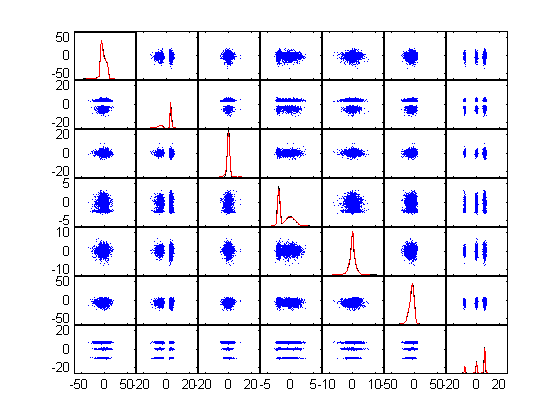
\includegraphics[width=4in,height=3.2in]{Fig/seven_outer_product_scatter.png}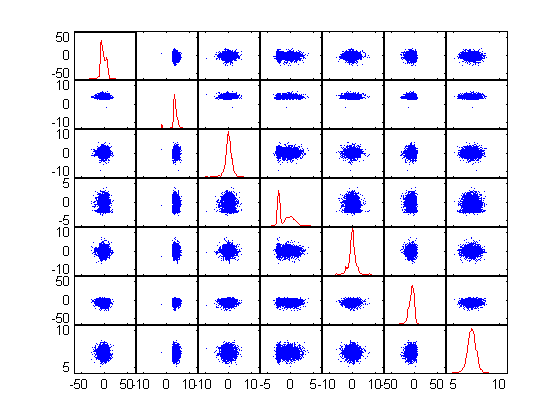
\includegraphics[width=4in,height=3.2in]{Fig/AIS_7d_outter_scatter.png}}
\end{tabular}
\caption{Seven dimensional outer product example. Left:posterior
samples produced by the proposed AAIS algorithm. Right:posterior
samples produced by the AMIS algorithm \citep{cappe2008ais}. In the
diagonal, the curves are kernel density estimates of the posterior
samples.} \label{fig:7D_scatter}
\end{figure}

Similarly as for example 1, we give a quantitative comparison for
the involved algorithms in Table \ref{comparison_7d}. We see that
again the proposed AAIS algorithm leads to much better results for
every comparison criterion.

\begin{table}
\begin{tabular}{c||c|c|c}
 & \ESS/$N$ & $\KL$ & Marginal likelihood: (true value:1) \\
\hline AMIS \citep{cappe2008ais}& 0.2454 & 10.8804 & $0.4675\pm0.0246$\\
\hline AAIS proposed here & 0.4948 & 0.4075  & $1.0011\pm0.0303$\\
\hline
\end{tabular}
\caption{Seven dimensional outer product example. Quantitative
Performance comparison}\label{comparison_7d}
\end{table}
